\documentclass[1p]{elsarticle_modified}
%\bibliographystyle{elsarticle-num}

%\usepackage[colorlinks]{hyperref}
%\usepackage{abbrmath_seonhwa} %\Abb, \Ascr, \Acal ,\Abf, \Afrak
\usepackage{amsfonts}
\usepackage{amssymb}
\usepackage{amsmath}
\usepackage{amsthm}
\usepackage{scalefnt}
\usepackage{amsbsy}
\usepackage{kotex}
\usepackage{caption}
\usepackage{subfig}
\usepackage{color}
\usepackage{graphicx}
\usepackage{xcolor} %% white, black, red, green, blue, cyan, magenta, yellow
\usepackage{float}
\usepackage{setspace}
\usepackage{hyperref}

\usepackage{tikz}
\usetikzlibrary{arrows}

\usepackage{multirow}
\usepackage{array} % fixed length table
\usepackage{hhline}

%%%%%%%%%%%%%%%%%%%%%
\makeatletter
\renewcommand*\env@matrix[1][\arraystretch]{%
	\edef\arraystretch{#1}%
	\hskip -\arraycolsep
	\let\@ifnextchar\new@ifnextchar
	\array{*\c@MaxMatrixCols c}}
\makeatother %https://tex.stackexchange.com/questions/14071/how-can-i-increase-the-line-spacing-in-a-matrix
%%%%%%%%%%%%%%%

\usepackage[normalem]{ulem}

\newcommand{\msout}[1]{\ifmmode\text{\sout{\ensuremath{#1}}}\else\sout{#1}\fi}
%SOURCE: \msout is \stkout macro in https://tex.stackexchange.com/questions/20609/strikeout-in-math-mode

\newcommand{\cancel}[1]{
	\ifmmode
	{\color{red}\msout{#1}}
	\else
	{\color{red}\sout{#1}}
	\fi
}

\newcommand{\add}[1]{
	{\color{blue}\uwave{#1}}
}

\newcommand{\replace}[2]{
	\ifmmode
	{\color{red}\msout{#1}}{\color{blue}\uwave{#2}}
	\else
	{\color{red}\sout{#1}}{\color{blue}\uwave{#2}}
	\fi
}

\newcommand{\Sol}{\mathcal{S}} %segment
\newcommand{\D}{D} %diagram
\newcommand{\A}{\mathcal{A}} %arc


%%%%%%%%%%%%%%%%%%%%%%%%%%%%%5 test

\def\sl{\operatorname{\textup{SL}}(2,\Cbb)}
\def\psl{\operatorname{\textup{PSL}}(2,\Cbb)}
\def\quan{\mkern 1mu \triangleright \mkern 1mu}

\theoremstyle{definition}
\newtheorem{thm}{Theorem}[section]
\newtheorem{prop}[thm]{Proposition}
\newtheorem{lem}[thm]{Lemma}
\newtheorem{ques}[thm]{Question}
\newtheorem{cor}[thm]{Corollary}
\newtheorem{defn}[thm]{Definition}
\newtheorem{exam}[thm]{Example}
\newtheorem{rmk}[thm]{Remark}
\newtheorem{alg}[thm]{Algorithm}

\newcommand{\I}{\sqrt{-1}}
\begin{document}

%\begin{frontmatter}
%
%\title{Boundary parabolic representations of knots up to 8 crossings}
%
%%% Group authors per affiliation:
%\author{Yunhi Cho} 
%\address{Department of Mathematics, University of Seoul, Seoul, Korea}
%\ead{yhcho@uos.ac.kr}
%
%
%\author{Seonhwa Kim} %\fnref{s_kim}}
%\address{Center for Geometry and Physics, Institute for Basic Science, Pohang, 37673, Korea}
%\ead{ryeona17@ibs.re.kr}
%
%\author{Hyuk Kim}
%\address{Department of Mathematical Sciences, Seoul National University, Seoul 08826, Korea}
%\ead{hyukkim@snu.ac.kr}
%
%\author{Seokbeom Yoon}
%\address{Department of Mathematical Sciences, Seoul National University, Seoul, 08826,  Korea}
%\ead{sbyoon15@snu.ac.kr}
%
%\begin{abstract}
%We find all boundary parabolic representation of knots up to 8 crossings.
%
%\end{abstract}
%\begin{keyword}
%    \MSC[2010] 57M25 
%\end{keyword}
%
%\end{frontmatter}

%\linenumbers
%\tableofcontents
%
\newcommand\colored[1]{\textcolor{white}{\rule[-0.35ex]{0.8em}{1.4ex}}\kern-0.8em\color{red} #1}%
%\newcommand\colored[1]{\textcolor{white}{ #1}\kern-2.17ex	\textcolor{white}{ #1}\kern-1.81ex	\textcolor{white}{ #1}\kern-2.15ex\color{red}#1	}

{\Large $\underline{11a_{237}~(K11a_{237})}$}

\setlength{\tabcolsep}{10pt}
\renewcommand{\arraystretch}{1.6}
\vspace{1cm}\begin{tabular}{m{100pt}>{\centering\arraybackslash}m{274pt}}
\multirow{5}{120pt}{
	\centering
	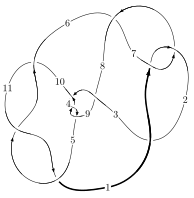
\includegraphics[width=112pt]{../../../GIT/diagram.site/Diagrams/png/486_11a_237.png}\\
\ \ \ A knot diagram\footnotemark}&
\allowdisplaybreaks
\textbf{Linearized knot diagam} \\
\cline{2-2}
 &
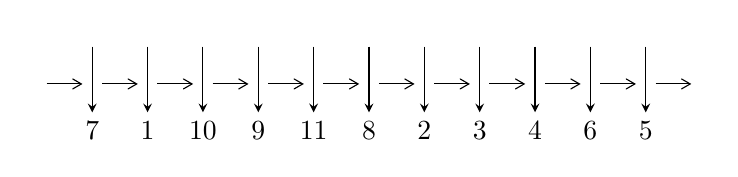
\begin{tikzpicture}[x=20pt, y=17pt]
	% nodes
	\node (C0) at (0, 0) {};
	\node (C1) at (1, 0) {};
	\node (C1U) at (1, +1) {};
	\node (C1D) at (1, -1) {7};

	\node (C2) at (2, 0) {};
	\node (C2U) at (2, +1) {};
	\node (C2D) at (2, -1) {1};

	\node (C3) at (3, 0) {};
	\node (C3U) at (3, +1) {};
	\node (C3D) at (3, -1) {10};

	\node (C4) at (4, 0) {};
	\node (C4U) at (4, +1) {};
	\node (C4D) at (4, -1) {9};

	\node (C5) at (5, 0) {};
	\node (C5U) at (5, +1) {};
	\node (C5D) at (5, -1) {11};

	\node (C6) at (6, 0) {};
	\node (C6U) at (6, +1) {};
	\node (C6D) at (6, -1) {8};

	\node (C7) at (7, 0) {};
	\node (C7U) at (7, +1) {};
	\node (C7D) at (7, -1) {2};

	\node (C8) at (8, 0) {};
	\node (C8U) at (8, +1) {};
	\node (C8D) at (8, -1) {3};

	\node (C9) at (9, 0) {};
	\node (C9U) at (9, +1) {};
	\node (C9D) at (9, -1) {4};

	\node (C10) at (10, 0) {};
	\node (C10U) at (10, +1) {};
	\node (C10D) at (10, -1) {6};

	\node (C11) at (11, 0) {};
	\node (C11U) at (11, +1) {};
	\node (C11D) at (11, -1) {5};
	\node (C12) at (12, 0) {};

	% arrows
	\draw[->,>={angle 60}]
	(C0) edge (C1) (C1) edge (C2) (C2) edge (C3) (C3) edge (C4) (C4) edge (C5) (C5) edge (C6) (C6) edge (C7) (C7) edge (C8) (C8) edge (C9) (C9) edge (C10) (C10) edge (C11) (C11) edge (C12) ;	\draw[->,>=stealth]
	(C1U) edge (C1D) (C2U) edge (C2D) (C3U) edge (C3D) (C4U) edge (C4D) (C5U) edge (C5D) (C6U) edge (C6D) (C7U) edge (C7D) (C8U) edge (C8D) (C9U) edge (C9D) (C10U) edge (C10D) (C11U) edge (C11D) ;
	\end{tikzpicture} \\
\hhline{~~} \\& 
\textbf{Solving Sequence} \\ \cline{2-2} 
 &
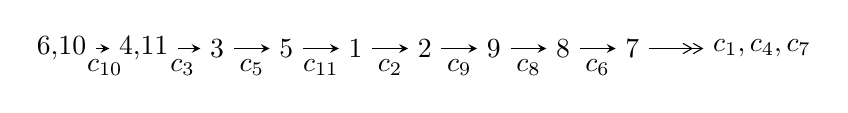
\begin{tikzpicture}[x=25pt, y=7pt]
	% node
	\node (A0) at (-1/8, 0) {6,10};
	\node (A1) at (17/16, 0) {4,11};
	\node (A2) at (17/8, 0) {3};
	\node (A3) at (25/8, 0) {5};
	\node (A4) at (33/8, 0) {1};
	\node (A5) at (41/8, 0) {2};
	\node (A6) at (49/8, 0) {9};
	\node (A7) at (57/8, 0) {8};
	\node (A8) at (65/8, 0) {7};
	\node (C1) at (1/2, -1) {$c_{10}$};
	\node (C2) at (13/8, -1) {$c_{3}$};
	\node (C3) at (21/8, -1) {$c_{5}$};
	\node (C4) at (29/8, -1) {$c_{11}$};
	\node (C5) at (37/8, -1) {$c_{2}$};
	\node (C6) at (45/8, -1) {$c_{9}$};
	\node (C7) at (53/8, -1) {$c_{8}$};
	\node (C8) at (61/8, -1) {$c_{6}$};
	\node (A9) at (10, 0) {$c_{1},c_{4},c_{7}$};

	% edge
	\draw[->,>=stealth]	
	(A0) edge (A1) (A1) edge (A2) (A2) edge (A3) (A3) edge (A4) (A4) edge (A5) (A5) edge (A6) (A6) edge (A7) (A7) edge (A8) ;
	\draw[->>,>={angle 60}]	
	(A8) edge (A9);
\end{tikzpicture} \\ 

\end{tabular} \\

\footnotetext{
The image of knot diagram is generated by the software ``\textbf{Draw programme}" developed by Andrew Bartholomew(\url{http://www.layer8.co.uk/maths/draw/index.htm\#Running-draw}), where we modified some parts for our purpose(\url{https://github.com/CATsTAILs/LinksPainter}).
}\phantom \\ \newline 
\centering \textbf{Ideals for irreducible components\footnotemark of $X_{\text{par}}$} 
 
\begin{align*}
I^u_{1}&=\langle 
b- u,\;u^{19}- u^{18}+\cdots+4 a+1,\;u^{20}+11 u^{18}+\cdots+3 u-1\rangle \\
I^u_{2}&=\langle 
-159484971 u^{29}+121594878 u^{28}+\cdots+95716253 b+570195911,\;- u^{29}+u^{28}+\cdots+a+6,\\
\phantom{I^u_{2}}&\phantom{= \langle  }u^{30}- u^{29}+\cdots-6 u+1\rangle \\
I^u_{3}&=\langle 
b+u,\;a^2-2 a u- a+u,\;u^2+1\rangle \\
\\
\end{align*}
\raggedright * 3 irreducible components of $\dim_{\mathbb{C}}=0$, with total 54 representations.\\
\footnotetext{All coefficients of polynomials are rational numbers. But the coefficients are sometimes approximated in decimal forms when there is not enough margin.}
\newpage
\renewcommand{\arraystretch}{1}
\centering \section*{I. $I^u_{1}= \langle b- u,\;u^{19}- u^{18}+\cdots+4 a+1,\;u^{20}+11 u^{18}+\cdots+3 u-1 \rangle$}
\flushleft \textbf{(i) Arc colorings}\\
\begin{tabular}{m{7pt} m{180pt} m{7pt} m{180pt} }
\flushright $a_{6}=$&$\begin{pmatrix}0\\u\end{pmatrix}$ \\
\flushright $a_{10}=$&$\begin{pmatrix}1\\0\end{pmatrix}$ \\
\flushright $a_{4}=$&$\begin{pmatrix}-\frac{1}{4} u^{19}+\frac{1}{4} u^{18}+\cdots+3 u-\frac{1}{4}\\u\end{pmatrix}$ \\
\flushright $a_{11}=$&$\begin{pmatrix}1\\u^2\end{pmatrix}$ \\
\flushright $a_{3}=$&$\begin{pmatrix}-\frac{1}{4} u^{19}+\frac{1}{4} u^{18}+\cdots+4 u-\frac{1}{4}\\u\end{pmatrix}$ \\
\flushright $a_{5}=$&$\begin{pmatrix}u\\u^3+u\end{pmatrix}$ \\
\flushright $a_{1}=$&$\begin{pmatrix}u^2+1\\u^4+2 u^2\end{pmatrix}$ \\
\flushright $a_{2}=$&$\begin{pmatrix}-\frac{1}{4} u^{19}+\frac{1}{4} u^{18}+\cdots+5 u-\frac{1}{4}\\\frac{1}{4} u^{19}-\frac{1}{4} u^{18}+\cdots+u^2+\frac{1}{4}\end{pmatrix}$ \\
\flushright $a_{9}=$&$\begin{pmatrix}-\frac{1}{4} u^{19}-\frac{1}{4} u^{18}+\cdots-\frac{1}{2} u+\frac{5}{4}\\- u^2\end{pmatrix}$ \\
\flushright $a_{8}=$&$\begin{pmatrix}-\frac{1}{4} u^{19}-\frac{1}{4} u^{18}+\cdots-\frac{1}{2} u+\frac{5}{4}\\- u^4-2 u^2\end{pmatrix}$ \\
\flushright $a_{7}=$&$\begin{pmatrix}\frac{1}{2} u^{19}+\frac{1}{2} u^{18}+\cdots+\frac{5}{2} u^2-2 u\\\frac{1}{4} u^{19}-\frac{1}{4} u^{18}+\cdots+u^2+\frac{1}{4}\end{pmatrix}$\\ \flushright $a_{7}=$&$\begin{pmatrix}\frac{1}{2} u^{19}+\frac{1}{2} u^{18}+\cdots+\frac{5}{2} u^2-2 u\\\frac{1}{4} u^{19}-\frac{1}{4} u^{18}+\cdots+u^2+\frac{1}{4}\end{pmatrix}$\\&\end{tabular}
\flushleft \textbf{(ii) Obstruction class $= -1$}\\~\\
\flushleft \textbf{(iii) Cusp Shapes $= -2 u^{19}-21 u^{17}-3 u^{16}-91 u^{15}-30 u^{14}-202 u^{13}-119 u^{12}-224 u^{11}-227 u^{10}-84 u^9-181 u^8+22 u^7+14 u^6-22 u^5+64 u^4-28 u^3-25 u^2+12 u-19$}\\~\\
\newpage\renewcommand{\arraystretch}{1}
\flushleft \textbf{(iv) u-Polynomials at the component}\newline \\
\begin{tabular}{m{50pt}|m{274pt}}
Crossings & \hspace{64pt}u-Polynomials at each crossing \\
\hline $$\begin{aligned}c_{1},c_{7}\end{aligned}$$&$\begin{aligned}
&u^{20}+3 u^{19}+\cdots-9 u-2
\end{aligned}$\\
\hline $$\begin{aligned}c_{2},c_{6}\end{aligned}$$&$\begin{aligned}
&u^{20}+7 u^{19}+\cdots+33 u+4
\end{aligned}$\\
\hline $$\begin{aligned}c_{3},c_{4},c_{5}\\c_{9},c_{10},c_{11}\end{aligned}$$&$\begin{aligned}
&u^{20}+11 u^{18}+\cdots-3 u-1
\end{aligned}$\\
\hline $$\begin{aligned}c_{8}\end{aligned}$$&$\begin{aligned}
&u^{20}-3 u^{19}+\cdots-48 u-32
\end{aligned}$\\
\hline
\end{tabular}\\~\\
\newpage\renewcommand{\arraystretch}{1}
\flushleft \textbf{(v) Riley Polynomials at the component}\newline \\
\begin{tabular}{m{50pt}|m{274pt}}
Crossings & \hspace{64pt}Riley Polynomials at each crossing \\
\hline $$\begin{aligned}c_{1},c_{7}\end{aligned}$$&$\begin{aligned}
&y^{20}-7 y^{19}+\cdots-33 y+4
\end{aligned}$\\
\hline $$\begin{aligned}c_{2},c_{6}\end{aligned}$$&$\begin{aligned}
&y^{20}+13 y^{19}+\cdots-561 y+16
\end{aligned}$\\
\hline $$\begin{aligned}c_{3},c_{4},c_{5}\\c_{9},c_{10},c_{11}\end{aligned}$$&$\begin{aligned}
&y^{20}+22 y^{19}+\cdots-5 y+1
\end{aligned}$\\
\hline $$\begin{aligned}c_{8}\end{aligned}$$&$\begin{aligned}
&y^{20}- y^{19}+\cdots+3328 y+1024
\end{aligned}$\\
\hline
\end{tabular}\\~\\
\newpage\flushleft \textbf{(vi) Complex Volumes and Cusp Shapes}
$$\begin{array}{c|c|c}  
\text{Solutions to }I^u_{1}& \I (\text{vol} + \sqrt{-1}CS) & \text{Cusp shape}\\
 \hline 
\begin{aligned}
u &= -0.711644 + 0.213665 I \\
a &= -0.992229 + 0.085972 I \\
b &= -0.711644 + 0.213665 I\end{aligned}
 & -0.77253 + 5.59830 I & -13.4954 - 6.8250 I \\ \hline\begin{aligned}
u &= -0.711644 - 0.213665 I \\
a &= -0.992229 - 0.085972 I \\
b &= -0.711644 - 0.213665 I\end{aligned}
 & -0.77253 - 5.59830 I & -13.4954 + 6.8250 I \\ \hline\begin{aligned}
u &= -0.714807\phantom{ +0.000000I} \\
a &= -0.946170\phantom{ +0.000000I} \\
b &= -0.714807\phantom{ +0.000000I}\end{aligned}
 & -4.75848\phantom{ +0.000000I} & -19.2850\phantom{ +0.000000I} \\ \hline\begin{aligned}
u &= \phantom{-}0.147507 + 1.344930 I \\
a &= \phantom{-}1.07486 - 2.87571 I \\
b &= \phantom{-}0.147507 + 1.344930 I\end{aligned}
 & \phantom{-}5.87096 + 0.28405 I & -5.48153 - 0.41216 I \\ \hline\begin{aligned}
u &= \phantom{-}0.147507 - 1.344930 I \\
a &= \phantom{-}1.07486 + 2.87571 I \\
b &= \phantom{-}0.147507 - 1.344930 I\end{aligned}
 & \phantom{-}5.87096 - 0.28405 I & -5.48153 + 0.41216 I \\ \hline\begin{aligned}
u &= \phantom{-}0.601815 + 0.228236 I \\
a &= \phantom{-}0.950028 + 0.149217 I \\
b &= \phantom{-}0.601815 + 0.228236 I\end{aligned}
 & \phantom{-}0.157185 - 0.414126 I & -12.01664 + 2.08787 I \\ \hline\begin{aligned}
u &= \phantom{-}0.601815 - 0.228236 I \\
a &= \phantom{-}0.950028 - 0.149217 I \\
b &= \phantom{-}0.601815 - 0.228236 I\end{aligned}
 & \phantom{-}0.157185 + 0.414126 I & -12.01664 - 2.08787 I \\ \hline\begin{aligned}
u &= \phantom{-}0.280299 + 1.365240 I \\
a &= \phantom{-}1.37177 - 2.14002 I \\
b &= \phantom{-}0.280299 + 1.365240 I\end{aligned}
 & \phantom{-}3.92725 - 7.17367 I & -8.70322 + 5.73165 I \\ \hline\begin{aligned}
u &= \phantom{-}0.280299 - 1.365240 I \\
a &= \phantom{-}1.37177 + 2.14002 I \\
b &= \phantom{-}0.280299 - 1.365240 I\end{aligned}
 & \phantom{-}3.92725 + 7.17367 I & -8.70322 - 5.73165 I \\ \hline\begin{aligned}
u &= -0.20040 + 1.40896 I \\
a &= -1.00049 - 2.38403 I \\
b &= -0.20040 + 1.40896 I\end{aligned}
 & \phantom{-}8.53664 + 4.27425 I & -2.38649 - 3.51536 I\\
 \hline 
 \end{array}$$\newpage$$\begin{array}{c|c|c}  
\text{Solutions to }I^u_{1}& \I (\text{vol} + \sqrt{-1}CS) & \text{Cusp shape}\\
 \hline 
\begin{aligned}
u &= -0.20040 - 1.40896 I \\
a &= -1.00049 + 2.38403 I \\
b &= -0.20040 - 1.40896 I\end{aligned}
 & \phantom{-}8.53664 - 4.27425 I & -2.38649 + 3.51536 I \\ \hline\begin{aligned}
u &= \phantom{-}0.35253 + 1.44249 I \\
a &= \phantom{-}1.15928 - 1.78353 I \\
b &= \phantom{-}0.35253 + 1.44249 I\end{aligned}
 & \phantom{-}9.8480 - 13.6547 I & -5.09222 + 8.08354 I \\ \hline\begin{aligned}
u &= \phantom{-}0.35253 - 1.44249 I \\
a &= \phantom{-}1.15928 + 1.78353 I \\
b &= \phantom{-}0.35253 - 1.44249 I\end{aligned}
 & \phantom{-}9.8480 + 13.6547 I & -5.09222 - 8.08354 I \\ \hline\begin{aligned}
u &= -0.32179 + 1.45317 I \\
a &= -1.09427 - 1.86772 I \\
b &= -0.32179 + 1.45317 I\end{aligned}
 & \phantom{-}11.02130 + 7.69202 I & -3.25100 - 3.40395 I \\ \hline\begin{aligned}
u &= -0.32179 - 1.45317 I \\
a &= -1.09427 + 1.86772 I \\
b &= -0.32179 - 1.45317 I\end{aligned}
 & \phantom{-}11.02130 - 7.69202 I & -3.25100 + 3.40395 I \\ \hline\begin{aligned}
u &= \phantom{-}0.074422 + 0.475930 I \\
a &= \phantom{-}0.299691 + 1.194600 I \\
b &= \phantom{-}0.074422 + 0.475930 I\end{aligned}
 & \phantom{-}1.45151 - 2.34993 I & -9.21397 + 4.74077 I \\ \hline\begin{aligned}
u &= \phantom{-}0.074422 - 0.475930 I \\
a &= \phantom{-}0.299691 - 1.194600 I \\
b &= \phantom{-}0.074422 - 0.475930 I\end{aligned}
 & \phantom{-}1.45151 + 2.34993 I & -9.21397 - 4.74077 I \\ \hline\begin{aligned}
u &= -0.02313 + 1.54067 I \\
a &= -0.08257 - 2.23973 I \\
b &= -0.02313 + 1.54067 I\end{aligned}
 & \phantom{-}15.2534 + 3.0855 I & -1.70716 - 2.62885 I \\ \hline\begin{aligned}
u &= -0.02313 - 1.54067 I \\
a &= -0.08257 + 2.23973 I \\
b &= -0.02313 - 1.54067 I\end{aligned}
 & \phantom{-}15.2534 - 3.0855 I & -1.70716 + 2.62885 I \\ \hline\begin{aligned}
u &= \phantom{-}0.315603\phantom{ +0.000000I} \\
a &= \phantom{-}0.574029\phantom{ +0.000000I} \\
b &= \phantom{-}0.315603\phantom{ +0.000000I}\end{aligned}
 & -0.553031\phantom{ +0.000000I} & -18.0200\phantom{ +0.000000I}\\
 \hline 
 \end{array}$$\newpage\newpage\renewcommand{\arraystretch}{1}
\centering \section*{II. $I^u_{2}= \langle -1.59\times10^{8} u^{29}+1.22\times10^{8} u^{28}+\cdots+9.57\times10^{7} b+5.70\times10^{8},\;- u^{29}+u^{28}+\cdots+a+6,\;u^{30}- u^{29}+\cdots-6 u+1 \rangle$}
\flushleft \textbf{(i) Arc colorings}\\
\begin{tabular}{m{7pt} m{180pt} m{7pt} m{180pt} }
\flushright $a_{6}=$&$\begin{pmatrix}0\\u\end{pmatrix}$ \\
\flushright $a_{10}=$&$\begin{pmatrix}1\\0\end{pmatrix}$ \\
\flushright $a_{4}=$&$\begin{pmatrix}u^{29}- u^{28}+\cdots+10 u-6\\1.66623 u^{29}-1.27037 u^{28}+\cdots+17.4027 u-5.95715\end{pmatrix}$ \\
\flushright $a_{11}=$&$\begin{pmatrix}1\\u^2\end{pmatrix}$ \\
\flushright $a_{3}=$&$\begin{pmatrix}2.66623 u^{29}-2.27037 u^{28}+\cdots+27.4027 u-11.9571\\1.66623 u^{29}-1.27037 u^{28}+\cdots+17.4027 u-5.95715\end{pmatrix}$ \\
\flushright $a_{5}=$&$\begin{pmatrix}u\\u^3+u\end{pmatrix}$ \\
\flushright $a_{1}=$&$\begin{pmatrix}u^2+1\\u^4+2 u^2\end{pmatrix}$ \\
\flushright $a_{2}=$&$\begin{pmatrix}4.72929 u^{29}-3.69976 u^{28}+\cdots+46.3017 u-17.7300\\2.22042 u^{29}-1.73024 u^{28}+\cdots+21.0519 u-7.17018\end{pmatrix}$ \\
\flushright $a_{9}=$&$\begin{pmatrix}5.95715 u^{29}-4.29092 u^{28}+\cdots+56.4198 u-17.3402\\0.395859 u^{29}+0.105883 u^{28}+\cdots+4.04021 u-0.666227\end{pmatrix}$ \\
\flushright $a_{8}=$&$\begin{pmatrix}5.19351 u^{29}-3.62763 u^{28}+\cdots+49.7650 u-14.1723\\-0.367778 u^{29}+0.769175 u^{28}+\cdots-2.61459 u+1.50174\end{pmatrix}$ \\
\flushright $a_{7}=$&$\begin{pmatrix}-6.74902 u^{29}+4.86232 u^{28}+\cdots-65.5259 u+23.3729\\-2.01973 u^{29}+1.16256 u^{28}+\cdots-17.2242 u+5.64291\end{pmatrix}$\\ \flushright $a_{7}=$&$\begin{pmatrix}-6.74902 u^{29}+4.86232 u^{28}+\cdots-65.5259 u+23.3729\\-2.01973 u^{29}+1.16256 u^{28}+\cdots-17.2242 u+5.64291\end{pmatrix}$\\&\end{tabular}
\flushleft \textbf{(ii) Obstruction class $= -1$}\\~\\
\flushleft \textbf{(iii) Cusp Shapes $= \frac{583799292}{95716253} u^{29}-\frac{406184408}{95716253} u^{28}+\cdots+\frac{4386525380}{95716253} u-\frac{2570388306}{95716253}$}\\~\\
\newpage\renewcommand{\arraystretch}{1}
\flushleft \textbf{(iv) u-Polynomials at the component}\newline \\
\begin{tabular}{m{50pt}|m{274pt}}
Crossings & \hspace{64pt}u-Polynomials at each crossing \\
\hline $$\begin{aligned}c_{1},c_{7}\end{aligned}$$&$\begin{aligned}
&(u^{15}- u^{14}+\cdots+2 u-1)^{2}
\end{aligned}$\\
\hline $$\begin{aligned}c_{2},c_{6}\end{aligned}$$&$\begin{aligned}
&(u^{15}+5 u^{14}+\cdots+12 u^3+1)^{2}
\end{aligned}$\\
\hline $$\begin{aligned}c_{3},c_{4},c_{5}\\c_{9},c_{10},c_{11}\end{aligned}$$&$\begin{aligned}
&u^{30}+u^{29}+\cdots+6 u+1
\end{aligned}$\\
\hline $$\begin{aligned}c_{8}\end{aligned}$$&$\begin{aligned}
&(u^{15}+u^{14}+\cdots-4 u-1)^{2}
\end{aligned}$\\
\hline
\end{tabular}\\~\\
\newpage\renewcommand{\arraystretch}{1}
\flushleft \textbf{(v) Riley Polynomials at the component}\newline \\
\begin{tabular}{m{50pt}|m{274pt}}
Crossings & \hspace{64pt}Riley Polynomials at each crossing \\
\hline $$\begin{aligned}c_{1},c_{7}\end{aligned}$$&$\begin{aligned}
&(y^{15}-5 y^{14}+\cdots+12 y^3-1)^{2}
\end{aligned}$\\
\hline $$\begin{aligned}c_{2},c_{6}\end{aligned}$$&$\begin{aligned}
&(y^{15}+11 y^{14}+\cdots-84 y^2-1)^{2}
\end{aligned}$\\
\hline $$\begin{aligned}c_{3},c_{4},c_{5}\\c_{9},c_{10},c_{11}\end{aligned}$$&$\begin{aligned}
&y^{30}+23 y^{29}+\cdots-16 y+1
\end{aligned}$\\
\hline $$\begin{aligned}c_{8}\end{aligned}$$&$\begin{aligned}
&(y^{15}- y^{14}+\cdots+16 y-1)^{2}
\end{aligned}$\\
\hline
\end{tabular}\\~\\
\newpage\flushleft \textbf{(vi) Complex Volumes and Cusp Shapes}
$$\begin{array}{c|c|c}  
\text{Solutions to }I^u_{2}& \I (\text{vol} + \sqrt{-1}CS) & \text{Cusp shape}\\
 \hline 
\begin{aligned}
u &= -0.171252 + 1.009920 I \\
a &= \phantom{-}0.163210 + 0.962498 I \\
b &= \phantom{-}0.318180 + 0.052816 I\end{aligned}
 & \phantom{-}1.46912 - 2.07402 I & -11.82822 + 2.67122 I \\ \hline\begin{aligned}
u &= -0.171252 - 1.009920 I \\
a &= \phantom{-}0.163210 - 0.962498 I \\
b &= \phantom{-}0.318180 - 0.052816 I\end{aligned}
 & \phantom{-}1.46912 + 2.07402 I & -11.82822 - 2.67122 I \\ \hline\begin{aligned}
u &= -0.607011 + 0.856391 I \\
a &= \phantom{-}0.550893 + 0.777218 I \\
b &= -0.108390 - 1.374740 I\end{aligned}
 & \phantom{-}6.82325 + 1.50523 I & -3.84867 - 2.74048 I \\ \hline\begin{aligned}
u &= -0.607011 - 0.856391 I \\
a &= \phantom{-}0.550893 - 0.777218 I \\
b &= -0.108390 + 1.374740 I\end{aligned}
 & \phantom{-}6.82325 - 1.50523 I & -3.84867 + 2.74048 I \\ \hline\begin{aligned}
u &= \phantom{-}0.879105 + 0.290763 I \\
a &= -1.025350 + 0.339134 I \\
b &= -0.28507 - 1.38638 I\end{aligned}
 & \phantom{-}4.31617 - 9.21780 I & -8.14540 + 7.39135 I \\ \hline\begin{aligned}
u &= \phantom{-}0.879105 - 0.290763 I \\
a &= -1.025350 - 0.339134 I \\
b &= -0.28507 + 1.38638 I\end{aligned}
 & \phantom{-}4.31617 + 9.21780 I & -8.14540 - 7.39135 I \\ \hline\begin{aligned}
u &= -0.836240 + 0.341718 I \\
a &= \phantom{-}1.024720 + 0.418737 I \\
b &= \phantom{-}0.241243 - 1.382540 I\end{aligned}
 & \phantom{-}5.27292 + 3.51852 I & -6.28698 - 2.59027 I \\ \hline\begin{aligned}
u &= -0.836240 - 0.341718 I \\
a &= \phantom{-}1.024720 - 0.418737 I \\
b &= \phantom{-}0.241243 + 1.382540 I\end{aligned}
 & \phantom{-}5.27292 - 3.51852 I & -6.28698 + 2.59027 I \\ \hline\begin{aligned}
u &= \phantom{-}0.587196 + 0.946781 I \\
a &= -0.473090 + 0.762799 I \\
b &= \phantom{-}0.171749 - 1.369410 I\end{aligned}
 & \phantom{-}6.30676 + 4.09199 I & -4.95573 - 3.15094 I \\ \hline\begin{aligned}
u &= \phantom{-}0.587196 - 0.946781 I \\
a &= -0.473090 - 0.762799 I \\
b &= \phantom{-}0.171749 + 1.369410 I\end{aligned}
 & \phantom{-}6.30676 - 4.09199 I & -4.95573 + 3.15094 I\\
 \hline 
 \end{array}$$\newpage$$\begin{array}{c|c|c}  
\text{Solutions to }I^u_{2}& \I (\text{vol} + \sqrt{-1}CS) & \text{Cusp shape}\\
 \hline 
\begin{aligned}
u &= \phantom{-}0.269205 + 1.103370 I \\
a &= -0.208705 + 0.855397 I \\
b &= \phantom{-}0.269205 - 1.103370 I\end{aligned}
 & \phantom{-}1.86559\phantom{ +0.000000I} & -10.56339 + 0. I\phantom{ +0.000000I} \\ \hline\begin{aligned}
u &= \phantom{-}0.269205 - 1.103370 I \\
a &= -0.208705 - 0.855397 I \\
b &= \phantom{-}0.269205 + 1.103370 I\end{aligned}
 & \phantom{-}1.86559\phantom{ +0.000000I} & -10.56339 + 0. I\phantom{ +0.000000I} \\ \hline\begin{aligned}
u &= \phantom{-}0.119824 + 1.236680 I \\
a &= -0.077620 + 0.801099 I \\
b &= -0.505429 - 0.368881 I\end{aligned}
 & \phantom{-}2.93870 - 1.66084 I & -6.48958 + 3.96405 I \\ \hline\begin{aligned}
u &= \phantom{-}0.119824 - 1.236680 I \\
a &= -0.077620 - 0.801099 I \\
b &= -0.505429 + 0.368881 I\end{aligned}
 & \phantom{-}2.93870 + 1.66084 I & -6.48958 - 3.96405 I \\ \hline\begin{aligned}
u &= \phantom{-}0.706910 + 0.161570 I \\
a &= -1.344380 + 0.307269 I \\
b &= -0.280017 - 1.247240 I\end{aligned}
 & -0.91830 - 3.60340 I & -14.1637 + 4.4767 I \\ \hline\begin{aligned}
u &= \phantom{-}0.706910 - 0.161570 I \\
a &= -1.344380 - 0.307269 I \\
b &= -0.280017 + 1.247240 I\end{aligned}
 & -0.91830 + 3.60340 I & -14.1637 - 4.4767 I \\ \hline\begin{aligned}
u &= -0.280017 + 1.247240 I \\
a &= \phantom{-}0.171369 + 0.763299 I \\
b &= \phantom{-}0.706910 - 0.161570 I\end{aligned}
 & -0.91830 + 3.60340 I & -14.1637 - 4.4767 I \\ \hline\begin{aligned}
u &= -0.280017 - 1.247240 I \\
a &= \phantom{-}0.171369 - 0.763299 I \\
b &= \phantom{-}0.706910 + 0.161570 I\end{aligned}
 & -0.91830 - 3.60340 I & -14.1637 + 4.4767 I \\ \hline\begin{aligned}
u &= -0.505429 + 0.368881 I \\
a &= \phantom{-}1.29090 + 0.94215 I \\
b &= \phantom{-}0.119824 - 1.236680 I\end{aligned}
 & \phantom{-}2.93870 + 1.66084 I & -6.48958 - 3.96405 I \\ \hline\begin{aligned}
u &= -0.505429 - 0.368881 I \\
a &= \phantom{-}1.29090 - 0.94215 I \\
b &= \phantom{-}0.119824 + 1.236680 I\end{aligned}
 & \phantom{-}2.93870 - 1.66084 I & -6.48958 + 3.96405 I\\
 \hline 
 \end{array}$$\newpage$$\begin{array}{c|c|c}  
\text{Solutions to }I^u_{2}& \I (\text{vol} + \sqrt{-1}CS) & \text{Cusp shape}\\
 \hline 
\begin{aligned}
u &= -0.108390 + 1.374740 I \\
a &= \phantom{-}0.056998 + 0.722915 I \\
b &= -0.607011 - 0.856391 I\end{aligned}
 & \phantom{-}6.82325 - 1.50523 I & -3.84867 + 2.74048 I \\ \hline\begin{aligned}
u &= -0.108390 - 1.374740 I \\
a &= \phantom{-}0.056998 - 0.722915 I \\
b &= -0.607011 + 0.856391 I\end{aligned}
 & \phantom{-}6.82325 + 1.50523 I & -3.84867 - 2.74048 I \\ \hline\begin{aligned}
u &= \phantom{-}0.171749 + 1.369410 I \\
a &= -0.090167 + 0.718933 I \\
b &= \phantom{-}0.587196 - 0.946781 I\end{aligned}
 & \phantom{-}6.30676 - 4.09199 I & -4.95573 + 3.15094 I \\ \hline\begin{aligned}
u &= \phantom{-}0.171749 - 1.369410 I \\
a &= -0.090167 - 0.718933 I \\
b &= \phantom{-}0.587196 + 0.946781 I\end{aligned}
 & \phantom{-}6.30676 + 4.09199 I & -4.95573 - 3.15094 I \\ \hline\begin{aligned}
u &= \phantom{-}0.241243 + 1.382540 I \\
a &= -0.122482 + 0.701932 I \\
b &= -0.836240 - 0.341718 I\end{aligned}
 & \phantom{-}5.27292 - 3.51852 I & -6.28698 + 2.59027 I \\ \hline\begin{aligned}
u &= \phantom{-}0.241243 - 1.382540 I \\
a &= -0.122482 - 0.701932 I \\
b &= -0.836240 + 0.341718 I\end{aligned}
 & \phantom{-}5.27292 + 3.51852 I & -6.28698 - 2.59027 I \\ \hline\begin{aligned}
u &= -0.28507 + 1.38638 I \\
a &= \phantom{-}0.142301 + 0.692043 I \\
b &= \phantom{-}0.879105 - 0.290763 I\end{aligned}
 & \phantom{-}4.31617 + 9.21780 I & -8.14540 - 7.39135 I \\ \hline\begin{aligned}
u &= -0.28507 - 1.38638 I \\
a &= \phantom{-}0.142301 - 0.692043 I \\
b &= \phantom{-}0.879105 + 0.290763 I\end{aligned}
 & \phantom{-}4.31617 - 9.21780 I & -8.14540 + 7.39135 I \\ \hline\begin{aligned}
u &= \phantom{-}0.318180 + 0.052816 I \\
a &= -3.05860 + 0.50771 I \\
b &= -0.171252 + 1.009920 I\end{aligned}
 & \phantom{-}1.46912 - 2.07402 I & -11.82822 + 2.67122 I \\ \hline\begin{aligned}
u &= \phantom{-}0.318180 - 0.052816 I \\
a &= -3.05860 - 0.50771 I \\
b &= -0.171252 - 1.009920 I\end{aligned}
 & \phantom{-}1.46912 + 2.07402 I & -11.82822 - 2.67122 I\\
 \hline 
 \end{array}$$\newpage\newpage\renewcommand{\arraystretch}{1}
\centering \section*{III. $I^u_{3}= \langle b+u,\;a^2-2 a u- a+u,\;u^2+1 \rangle$}
\flushleft \textbf{(i) Arc colorings}\\
\begin{tabular}{m{7pt} m{180pt} m{7pt} m{180pt} }
\flushright $a_{6}=$&$\begin{pmatrix}0\\u\end{pmatrix}$ \\
\flushright $a_{10}=$&$\begin{pmatrix}1\\0\end{pmatrix}$ \\
\flushright $a_{4}=$&$\begin{pmatrix}a\\- u\end{pmatrix}$ \\
\flushright $a_{11}=$&$\begin{pmatrix}1\\-1\end{pmatrix}$ \\
\flushright $a_{3}=$&$\begin{pmatrix}a- u\\- u\end{pmatrix}$ \\
\flushright $a_{5}=$&$\begin{pmatrix}u\\0\end{pmatrix}$ \\
\flushright $a_{1}=$&$\begin{pmatrix}0\\-1\end{pmatrix}$ \\
\flushright $a_{2}=$&$\begin{pmatrix}a- u\\- a\end{pmatrix}$ \\
\flushright $a_{9}=$&$\begin{pmatrix}a u+1\\1\end{pmatrix}$ \\
\flushright $a_{8}=$&$\begin{pmatrix}a u+1\\1\end{pmatrix}$ \\
\flushright $a_{7}=$&$\begin{pmatrix}a u- u+1\\a\end{pmatrix}$\\ \flushright $a_{7}=$&$\begin{pmatrix}a u- u+1\\a\end{pmatrix}$\\&\end{tabular}
\flushleft \textbf{(ii) Obstruction class $= 1$}\\~\\
\flushleft \textbf{(iii) Cusp Shapes $= 4 a-4 u-8$}\\~\\
\newpage\renewcommand{\arraystretch}{1}
\flushleft \textbf{(iv) u-Polynomials at the component}\newline \\
\begin{tabular}{m{50pt}|m{274pt}}
Crossings & \hspace{64pt}u-Polynomials at each crossing \\
\hline $$\begin{aligned}c_{1},c_{7}\end{aligned}$$&$\begin{aligned}
&u^4- u^2+1
\end{aligned}$\\
\hline $$\begin{aligned}c_{2}\end{aligned}$$&$\begin{aligned}
&(u^2+u+1)^2
\end{aligned}$\\
\hline $$\begin{aligned}c_{3},c_{4},c_{5}\\c_{9},c_{10},c_{11}\end{aligned}$$&$\begin{aligned}
&(u^2+1)^2
\end{aligned}$\\
\hline $$\begin{aligned}c_{6}\end{aligned}$$&$\begin{aligned}
&(u^2- u+1)^2
\end{aligned}$\\
\hline $$\begin{aligned}c_{8}\end{aligned}$$&$\begin{aligned}
&u^4
\end{aligned}$\\
\hline
\end{tabular}\\~\\
\newpage\renewcommand{\arraystretch}{1}
\flushleft \textbf{(v) Riley Polynomials at the component}\newline \\
\begin{tabular}{m{50pt}|m{274pt}}
Crossings & \hspace{64pt}Riley Polynomials at each crossing \\
\hline $$\begin{aligned}c_{1},c_{7}\end{aligned}$$&$\begin{aligned}
&(y^2- y+1)^2
\end{aligned}$\\
\hline $$\begin{aligned}c_{2},c_{6}\end{aligned}$$&$\begin{aligned}
&(y^2+y+1)^2
\end{aligned}$\\
\hline $$\begin{aligned}c_{3},c_{4},c_{5}\\c_{9},c_{10},c_{11}\end{aligned}$$&$\begin{aligned}
&(y+1)^4
\end{aligned}$\\
\hline $$\begin{aligned}c_{8}\end{aligned}$$&$\begin{aligned}
&y^4
\end{aligned}$\\
\hline
\end{tabular}\\~\\
\newpage\flushleft \textbf{(vi) Complex Volumes and Cusp Shapes}
$$\begin{array}{c|c|c}  
\text{Solutions to }I^u_{3}& \I (\text{vol} + \sqrt{-1}CS) & \text{Cusp shape}\\
 \hline 
\begin{aligned}
u &= \phantom{-0.000000 -}1.000000 I \\
a &= \phantom{-}0.500000 + 0.133975 I \\
b &= \phantom{-0.000000 } -1.000000 I\end{aligned}
 & \phantom{-}3.28987 + 2.02988 I & -6.00000 - 3.46410 I \\ \hline\begin{aligned}
u &= \phantom{-0.000000 -}1.000000 I \\
a &= \phantom{-}0.50000 + 1.86603 I \\
b &= \phantom{-0.000000 } -1.000000 I\end{aligned}
 & \phantom{-}3.28987 - 2.02988 I & -6.00000 + 3.46410 I \\ \hline\begin{aligned}
u &= \phantom{-0.000000 } -1.000000 I \\
a &= \phantom{-}0.500000 - 0.133975 I \\
b &= \phantom{-0.000000 -}1.000000 I\end{aligned}
 & \phantom{-}3.28987 - 2.02988 I & -6.00000 + 3.46410 I \\ \hline\begin{aligned}
u &= \phantom{-0.000000 } -1.000000 I \\
a &= \phantom{-}0.50000 - 1.86603 I \\
b &= \phantom{-0.000000 -}1.000000 I\end{aligned}
 & \phantom{-}3.28987 + 2.02988 I & -6.00000 - 3.46410 I\\
 \hline 
 \end{array}$$\newpage
\newpage\renewcommand{\arraystretch}{1}
\centering \section*{ IV. u-Polynomials}
\begin{tabular}{m{50pt}|m{274pt}}
Crossings & \hspace{64pt}u-Polynomials at each crossing \\
\hline $$\begin{aligned}c_{1},c_{7}\end{aligned}$$&$\begin{aligned}
&(u^4- u^2+1)(u^{15}- u^{14}+\cdots+2 u-1)^{2}(u^{20}+3 u^{19}+\cdots-9 u-2)
\end{aligned}$\\
\hline $$\begin{aligned}c_{2}\end{aligned}$$&$\begin{aligned}
&((u^2+u+1)^2)(u^{15}+5 u^{14}+\cdots+12 u^3+1)^{2}\\
&\cdot(u^{20}+7 u^{19}+\cdots+33 u+4)
\end{aligned}$\\
\hline $$\begin{aligned}c_{3},c_{4},c_{5}\\c_{9},c_{10},c_{11}\end{aligned}$$&$\begin{aligned}
&((u^2+1)^2)(u^{20}+11 u^{18}+\cdots-3 u-1)(u^{30}+u^{29}+\cdots+6 u+1)
\end{aligned}$\\
\hline $$\begin{aligned}c_{6}\end{aligned}$$&$\begin{aligned}
&((u^2- u+1)^2)(u^{15}+5 u^{14}+\cdots+12 u^3+1)^{2}\\
&\cdot(u^{20}+7 u^{19}+\cdots+33 u+4)
\end{aligned}$\\
\hline $$\begin{aligned}c_{8}\end{aligned}$$&$\begin{aligned}
&u^4(u^{15}+u^{14}+\cdots-4 u-1)^{2}(u^{20}-3 u^{19}+\cdots-48 u-32)
\end{aligned}$\\
\hline
\end{tabular}\newpage\renewcommand{\arraystretch}{1}
\centering \section*{ V. Riley Polynomials}
\begin{tabular}{m{50pt}|m{274pt}}
Crossings & \hspace{64pt}Riley Polynomials at each crossing \\
\hline $$\begin{aligned}c_{1},c_{7}\end{aligned}$$&$\begin{aligned}
&((y^2- y+1)^2)(y^{15}-5 y^{14}+\cdots+12 y^3-1)^{2}\\
&\cdot(y^{20}-7 y^{19}+\cdots-33 y+4)
\end{aligned}$\\
\hline $$\begin{aligned}c_{2},c_{6}\end{aligned}$$&$\begin{aligned}
&((y^2+y+1)^2)(y^{15}+11 y^{14}+\cdots-84 y^2-1)^{2}\\
&\cdot(y^{20}+13 y^{19}+\cdots-561 y+16)
\end{aligned}$\\
\hline $$\begin{aligned}c_{3},c_{4},c_{5}\\c_{9},c_{10},c_{11}\end{aligned}$$&$\begin{aligned}
&((y+1)^4)(y^{20}+22 y^{19}+\cdots-5 y+1)(y^{30}+23 y^{29}+\cdots-16 y+1)
\end{aligned}$\\
\hline $$\begin{aligned}c_{8}\end{aligned}$$&$\begin{aligned}
&y^4(y^{15}- y^{14}+\cdots+16 y-1)^{2}(y^{20}-y^{19}+\cdots+3328 y+1024)
\end{aligned}$\\
\hline
\end{tabular}
\vskip 2pc
\end{document}